\documentclass[border=6pt,tikz]{standalone}
\usepackage{tikz}
\usepackage{amsmath,amssymb}
\usetikzlibrary{arrows.meta,positioning,fit,backgrounds,calc,shapes.geometric,decorations.pathreplacing,patterns}
\definecolor{ink}{HTML}{1B2430}
\definecolor{muted}{HTML}{6B7785}
\definecolor{accent}{HTML}{2F6FB5}
\definecolor{accent2}{HTML}{C1611F}
\definecolor{good}{HTML}{2E7D5B}
\definecolor{soft}{HTML}{EDF2F7}
\definecolor{soft2}{HTML}{FBEDE2}
\definecolor{soft3}{HTML}{E6F0E9}
\tikzset{
  box/.style={draw=ink,line width=.7pt,rounded corners=2pt,fill=soft,inner sep=4pt,align=center,font=\sffamily\small},
  boxa/.style={box,fill=soft2},
  boxb/.style={box,fill=soft3},
  plain/.style={align=center,font=\sffamily\small,text=ink},
  tiny/.style={align=center,font=\sffamily\scriptsize,text=muted},
  ar/.style={-{Stealth[length=2.4mm]},draw=ink,line width=.7pt},
  arm/.style={-{Stealth[length=2.4mm]},draw=muted,line width=.6pt,dashed},
  nd/.style={circle,draw=ink,line width=.7pt,fill=white,minimum size=7mm,inner sep=0pt,font=\sffamily\scriptsize},
  ndf/.style={nd,fill=soft},
  ndt/.style={nd,fill=soft2},
}

\begin{document}
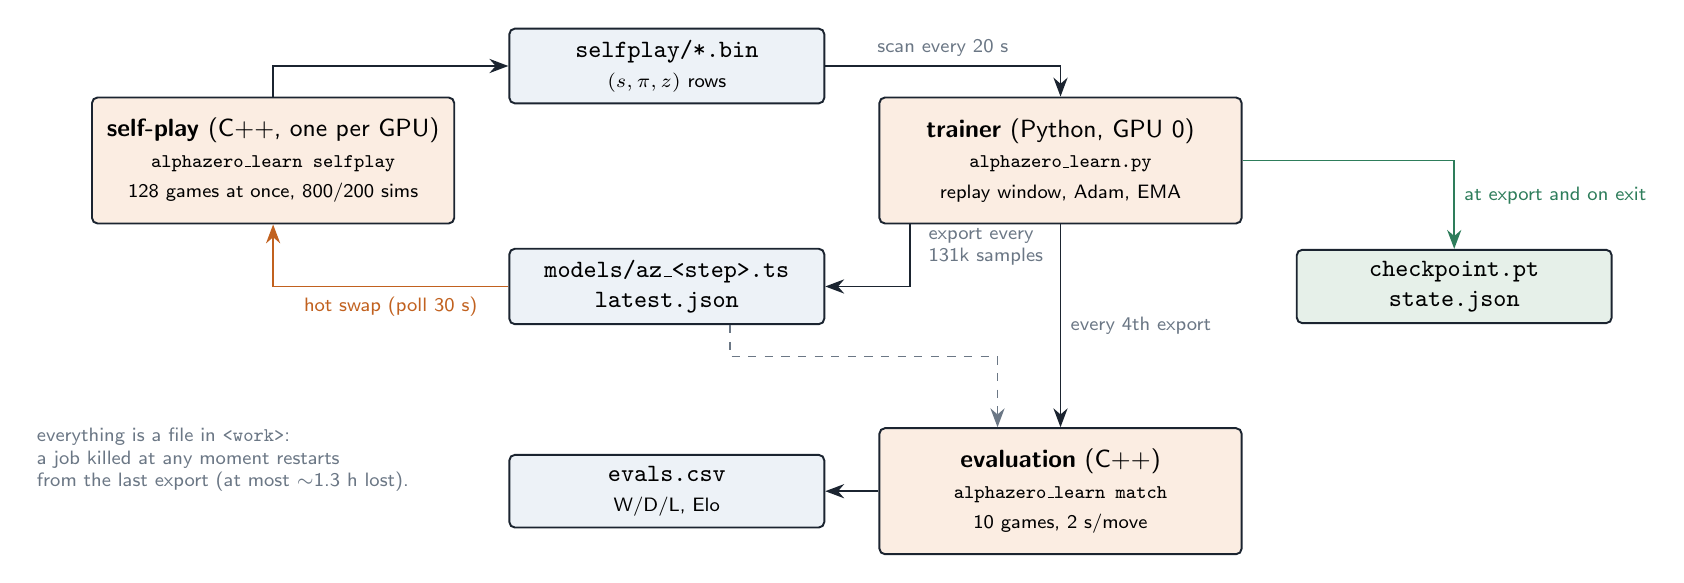
\begin{tikzpicture}[x=1mm,y=1mm]
  % processes
  \node[boxa,minimum width=46mm,minimum height=16mm] (sp) at (0,0)
    {\textbf{self-play} (C++, one per GPU)\\\scriptsize\texttt{alphazero\_learn selfplay}\\\scriptsize 128 games at once, 800/200 sims};
  \node[boxa,minimum width=46mm,minimum height=16mm] (tr) at (100,0)
    {\textbf{trainer} (Python, GPU 0)\\\scriptsize\texttt{alphazero\_learn.py}\\\scriptsize replay window, Adam, EMA};
  \node[boxa,minimum width=46mm,minimum height=16mm] (ev) at (100,-42)
    {\textbf{evaluation} (C++)\\\scriptsize\texttt{alphazero\_learn match}\\\scriptsize 10 games, 2 s/move};
  % files
  \node[box,minimum width=40mm] (data) at (50,12) {\texttt{selfplay/*.bin}\\\scriptsize $(s,\pi,z)$ rows};
  \node[box,minimum width=40mm] (models) at (50,-16) {\texttt{models/az\_<step>.ts}\\\texttt{latest.json}};
  \node[box,minimum width=40mm] (csv) at (50,-42) {\texttt{evals.csv}\\\scriptsize W/D/L, Elo};
  \node[boxb,minimum width=40mm] (ck) at (150,-16) {\texttt{checkpoint.pt}\\\texttt{state.json}};
  \draw[ar] (sp.north) |- (data.west);
  \draw[ar] (data.east) -| node[tiny,pos=.25,above]{scan every 20 s} (tr.north);
  \draw[ar] (tr.south west) ++(4,0) |- (models.east);
  \node[tiny,anchor=west,align=left] at (82,-11) {export every\\131k samples};
  \draw[ar,draw=accent2] (models.west) -| node[tiny,pos=.25,below,text=accent2]{hot swap (poll 30 s)} (sp.south);
  \draw[ar] (tr.south) -- node[tiny,right]{every 4th export} (ev.north);
  \draw[arm] (models.south) ++(8,0) -- ++(0,-4) -| ([xshift=-8mm]ev.north);
  \draw[ar] (ev.west) -- (csv.east);
  \draw[ar,draw=good] (tr.east) -| node[tiny,pos=.7,right,text=good]{at export and on exit} (ck.north);
  \node[tiny,text width=60mm,align=left] at (0,-38)
   {everything is a file in \texttt{<work>}:\\a job killed at any moment restarts\\from the last export (at most $\sim$1.3 h lost).};
\end{tikzpicture}
\end{document}
